\section{Тестирование}
    Ниже приведены результаты тестирования двух методов оптимизации на тестовых функциях, первый использует метод золотого сечения, для поиска минимума вдоль направления, а другой алгоритм Moore-Skelboe.

    \subsection*{Функция Растригина}

    \subsubsection*{График функции при $n=2$}
    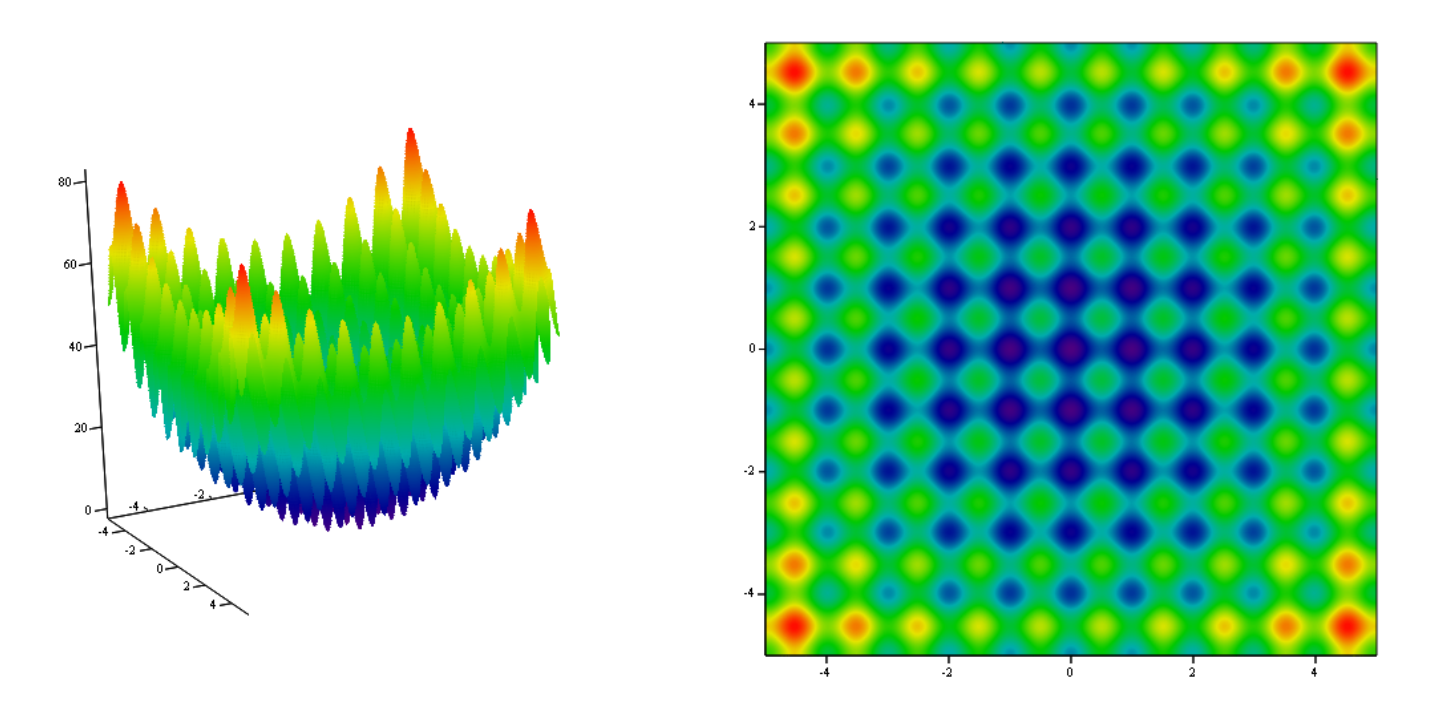
\includegraphics[width=16cm, height=8cm]{Rastrigin}

    \subsubsection*{Формула}
    \begin{gather*}
        f(x)=10 n+\sum_{i=1}^n\left(x_i^2-10 \cdot \cos \left(2 \pi \cdot x_i\right)\right)
    \end{gather*}

    \subsubsection*{Результаты тестирования}

    \begin{tabular}{ |p{2cm}|p{2cm}|p{3cm}|p{2cm}|p{4cm}|  }
        \hline
        n  & точность & метод         & время   & минимум                \\
        \hline
        5  & $10^-3$  & Golden ratio  & 2.22 ms & 4.974821275706137      \\\cline{2-5}
        & $10^-3$  & Moore-Skelboe & 178 ms  & 9.238348694395881e-05  \\
        \hline
        10 & $10^-3$  & Golden ratio  & 4.78 ms & 9.94964255141227       \\\cline{2-5}
        & $10^-3$  & Moore-Skelboe & 736 ms  & 0.00018476697390212848 \\
        \hline
        20 & $10^-3$  & Golden ratio  & 13.3 ms & 19.899285102824635     \\\cline{2-5}
        & $10^-3$  & Moore-Skelboe & 2.52 s  & 0.0003695339478184678  \\
        \hline
        30 & $10^-3$  & Golden ratio  & 24.1 ms & 29.84892765423696      \\\cline{2-5}
        & $10^-3$  & Moore-Skelboe & 5.38 s  & 0.0005543009217348072  \\
        \hline
        40 & $10^-3$  & Golden ratio  & 43.2 ms & 39.79857020564907      \\\cline{2-5}
        & $10^-3$  & Moore-Skelboe & 9.58 s  & 0.0007390678956511465  \\
        \hline
        50 & $10^-3$  & Golden ratio  & 58.8 ms & 49.748212757061154     \\\cline{2-5}
        & $10^-3$  & Moore-Skelboe & 14.9 s  & 0.0009238348695674858  \\
        \hline

    \end{tabular}

    \subsection*{Функция Растригина новгородская}

    \subsubsection*{График функции при $n=2$}
    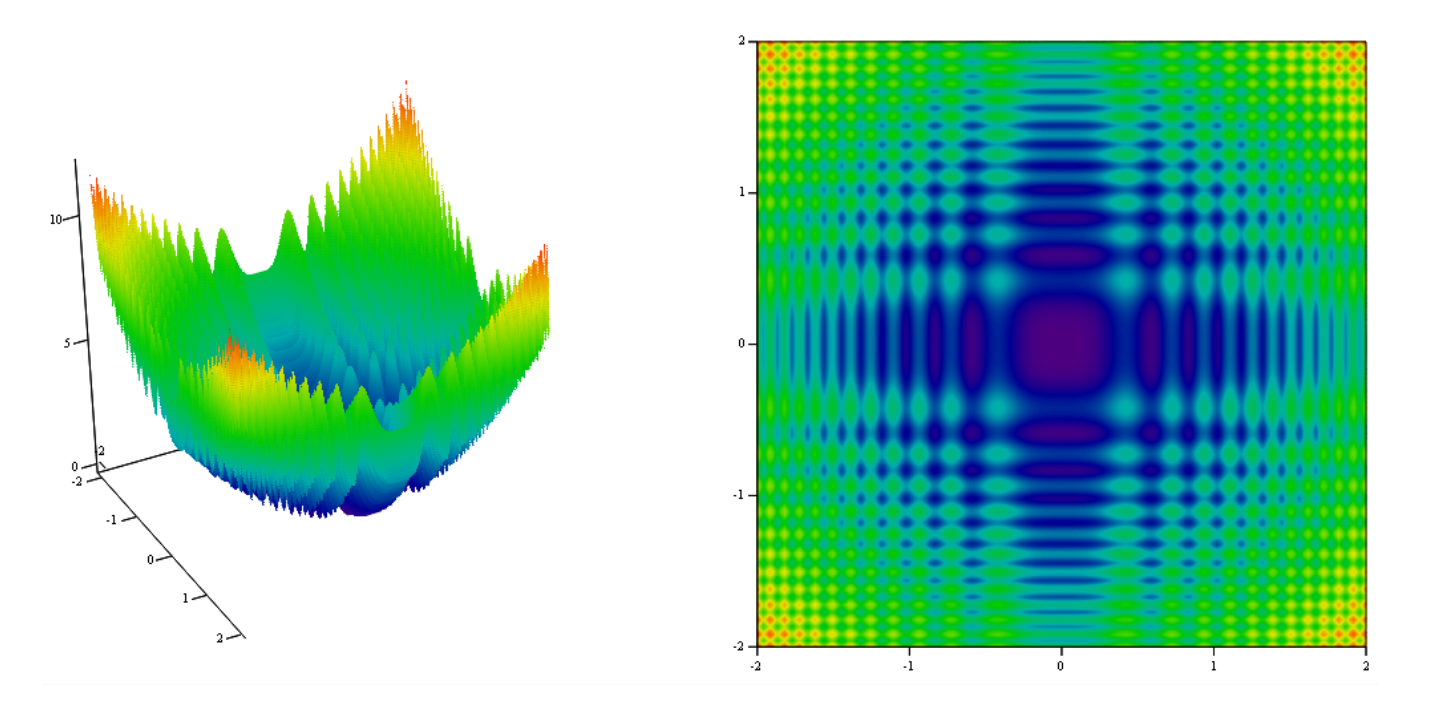
\includegraphics[width=16cm, height=8cm]{Rastrigin_new}

    \subsubsection*{Формула}
    \begin{gather*}
        f(x)=n+\sum_{i=1}^n\left(x_i^2-\cos \left(18 \cdot x_i^2\right)\right)
    \end{gather*}

    \subsubsection*{Результаты тестирования}

    \begin{tabular}{ |p{2cm}|p{2cm}|p{3cm}|p{2cm}|p{4cm}|  }
        \hline
        n  & точность & метод         & время   & значение              \\
        \hline
        5  & $10^-3$  & Golden ratio  & 1.36 ms & 1.542458003137213     \\\cline{2-5}
        & $10^-3$  & Moore-Skelboe & 151 ms  & 0.0007449817996270092 \\
        \hline
        10 & $10^-3$  & Golden ratio  & 5.18 ms & 3.0849160062744287    \\\cline{2-5}
        & $10^-3$  & Moore-Skelboe & 636 ms  & 0.0014899635992544624 \\
        \hline
        20 & $10^-3$  & Golden ratio  & 20.8 ms & 6.16983201254885      \\\cline{2-5}
        & $10^-3$  & Moore-Skelboe & 1.94 s  & 0.002979927198509369  \\
        \hline
        30 & $10^-3$  & Golden ratio  & 37 ms   & 9.254748018823253     \\\cline{2-5}
        & $10^-3$  & Moore-Skelboe & 4.54 s  & 0.0044698907977642754 \\
        \hline
        40 & $10^-3$  & Golden ratio  & 54.2 ms & 12.339664025097658    \\\cline{2-5}
        & $10^-3$  & Moore-Skelboe & 7.79 s  & 0.005959854397019182  \\
        \hline
        50 & $10^-3$  & Golden ratio  & 79.7 ms & 15.424580031372061    \\\cline{2-5}
        & $10^-3$  & Moore-Skelboe & 11.6 s  & 0.0074498179962740885 \\
        \hline

    \end{tabular}

    \subsection*{Функция Розенброка}

    \subsubsection*{График функции при $n=2$}
    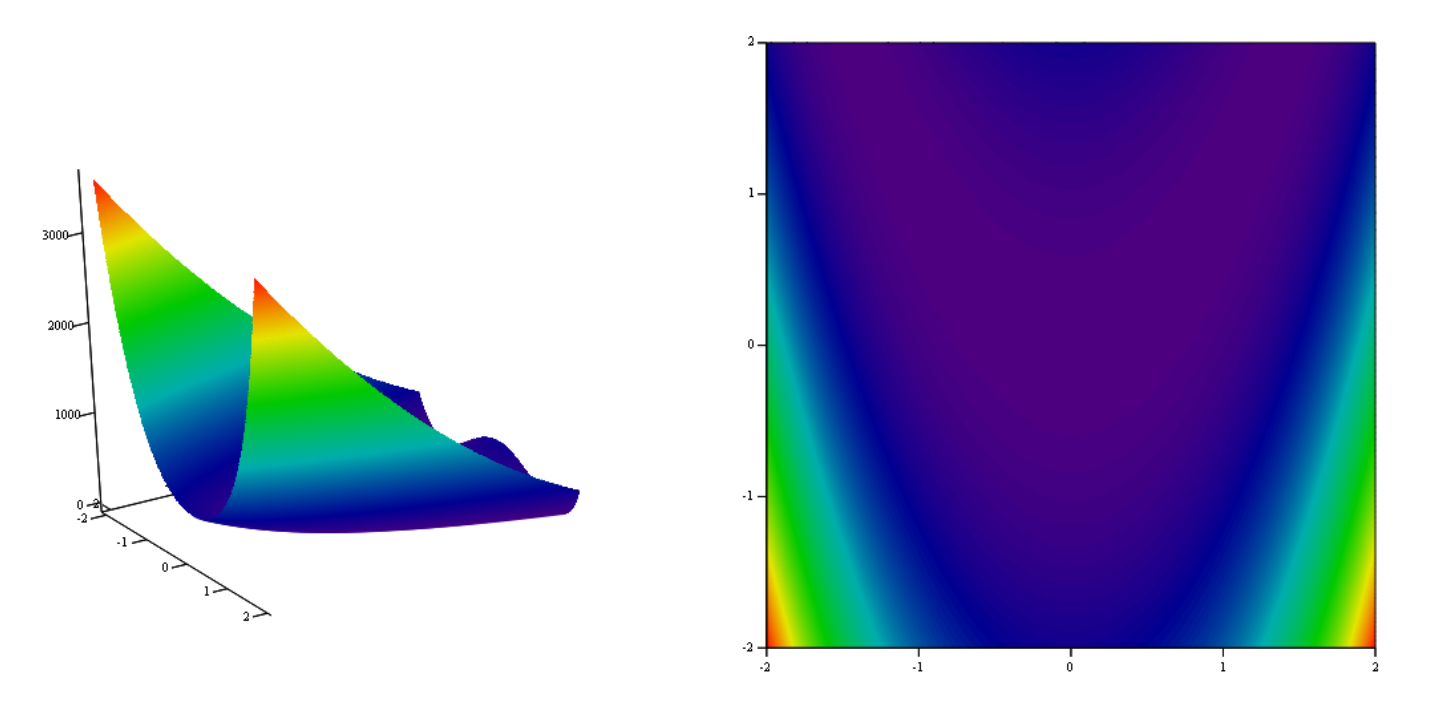
\includegraphics[width=16cm, height=8cm]{Rozenbrock}

    \subsubsection*{Формула}
    \begin{gather*}
        f(x)=\sum_{i=1}^{n-1}\left(100\left(x_{i+1}-x_i^2\right)^2+\left(1-x_i\right)^2\right)
    \end{gather*}

    \subsubsection*{Результаты тестирования}

    \begin{tabular}{ |p{2cm}|p{2cm}|p{3cm}|p{2cm}|p{4cm}|  }
        \hline
        n & точность & метод         & время   & значение            \\
        \hline
        2 & $10^-3$  & Golden ratio  & 1.12 ms & 0.16956582889643249 \\\cline{2-5}
        & $10^-3$  & Moore-Skelboe & 155 ms  & 0.16036252999621464 \\
        \hline
        3 & $10^-3$  & Golden ratio  & 5.95 ms & 0.259397310396006   \\\cline{2-5}
        & $10^-3$  & Moore-Skelboe & 3.99 s  & 0.11254106932659813 \\
        \hline
        4 & $10^-3$  & Golden ratio  & 17 ms   & 0.28064340055794645 \\\cline{2-5}
        & $10^-3$  & Moore-Skelboe & 8.75 s  & 0.11734786681147619 \\
        \hline
        5 & $10^-3$  & Golden ratio  & 27.3 ms & 0.2830939134564683  \\\cline{2-5}
        & $10^-3$  & Moore-Skelboe & 15.6 s  & 0.11851270446807871 \\
        \hline
        6 & $10^-3$  & Golden ratio  & 40.4 ms & 0.29047947563212634 \\\cline{2-5}
        & $10^-3$  & Moore-Skelboe & 24.5 s  & 0.11879389607067276 \\
        \hline
        7 & $10^-3$  & Golden ratio  & 49.2 ms & 0.29064024190256904 \\\cline{2-5}
        & $10^-3$  & Moore-Skelboe & 35.6 s  & 0.1136410373197746  \\
        \hline
        8 & $10^-3$  & Golden ratio  & 18.5 ms & 0.33244082803407593 \\\cline{2-5}
        & $10^-3$  & Moore-Skelboe & 41.7 s  & 0.14015453688727936 \\
        \hline

    \end{tabular}

    \subsection*{Функция Экли}

    \subsubsection*{График функции при $n=2$}
    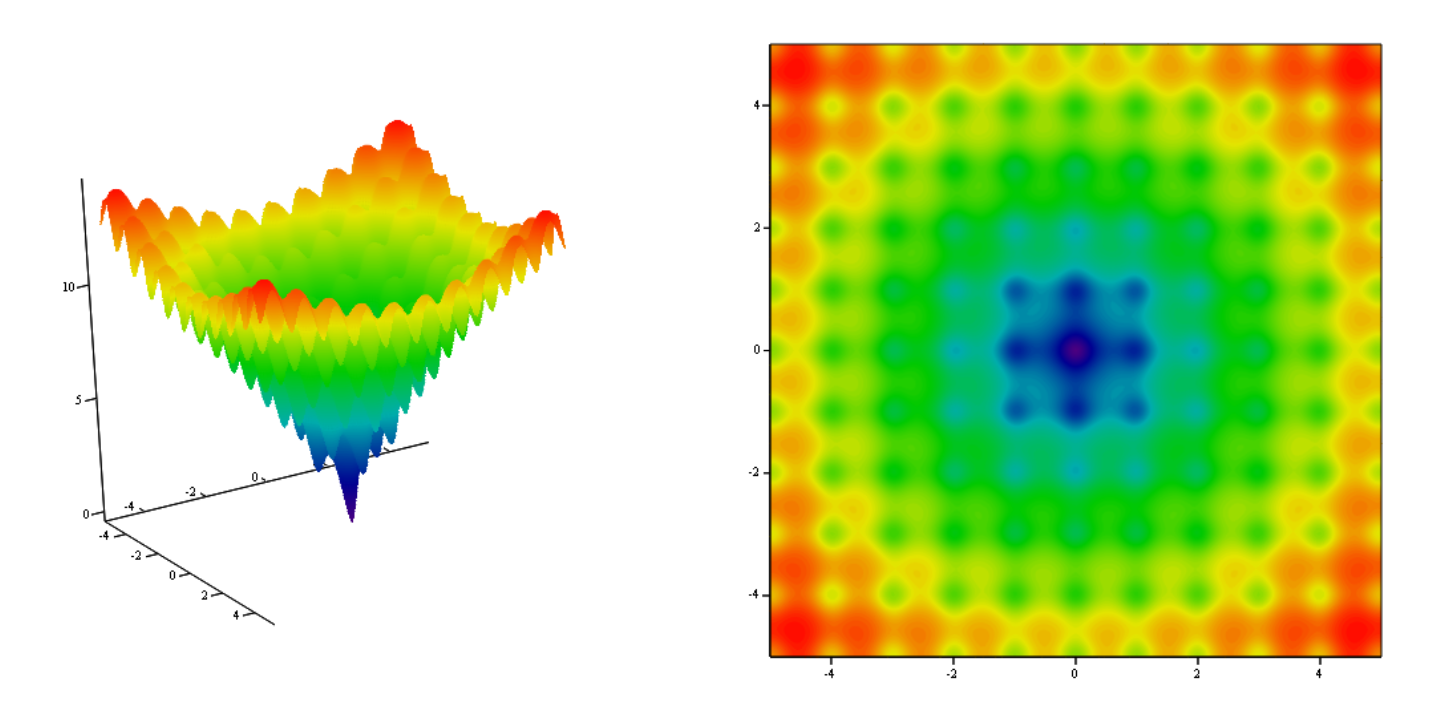
\includegraphics[width=16cm, height=8cm]{Ackley}

    \subsubsection*{Формула}
    \begin{gather*}
        f(x)=20+e-20 e^{-0.2 \sqrt{\frac{1}{n} \sum_{i=1}^n x_i^2}}-e^{\frac{1}{n} \sum_{i=1}^n \cos \left(2 \pi \cdot x_i\right)}
    \end{gather*}

    \subsubsection*{Результаты тестирования}

    \begin{tabular}{ |p{2cm}|p{2cm}|p{3cm}|p{2cm}|p{4cm}|  }
        \hline
        n  & точность & метод         & время   & значение               \\
        \hline
        5  & $10^-3$  & Golden ratio  & 2.41 ms & -4.440892098500626e-16 \\\cline{2-5}
        & $10^-3$  & Moore-Skelboe & 553 ms  & 0.0012256630393632229  \\
        \hline
        20 & $10^-3$  & Golden ratio  & 9.06 ms & 3.5744545080266543     \\\cline{2-5}
        & $10^-3$  & Moore-Skelboe & 1.35 s  & 0.0012256630393632229  \\
        \hline
        20 & $10^-3$  & Golden ratio  & 30.6 ms & 3.5744545080266543     \\\cline{2-5}
        & $10^-3$  & Moore-Skelboe & 3.41 s  & 0.0012256630393632229  \\
        \hline
        30 & $10^-3$  & Golden ratio  & 58.5 ms & 3.574454508026655      \\\cline{2-5}
        & $10^-3$  & Moore-Skelboe & 6.23 s  & 0.0012256630393645551  \\
        \hline
        40 & $10^-3$  & Golden ratio  & 84.1 ms & 3.574454508026654      \\\cline{2-5}
        & $10^-3$  & Moore-Skelboe & 10.6 s  & 0.0012256630393632229  \\
        \hline
        50 & $10^-3$  & Golden ratio  & 124 ms  & 3.5744545080266525     \\\cline{2-5}
        & $10^-3$  & Moore-Skelboe & 14.9 s  & 0.0012256630393618906  \\
        \hline

    \end{tabular}

    \subsection*{Функция Гриванка}

    \subsubsection*{График функции при $n=2$}
    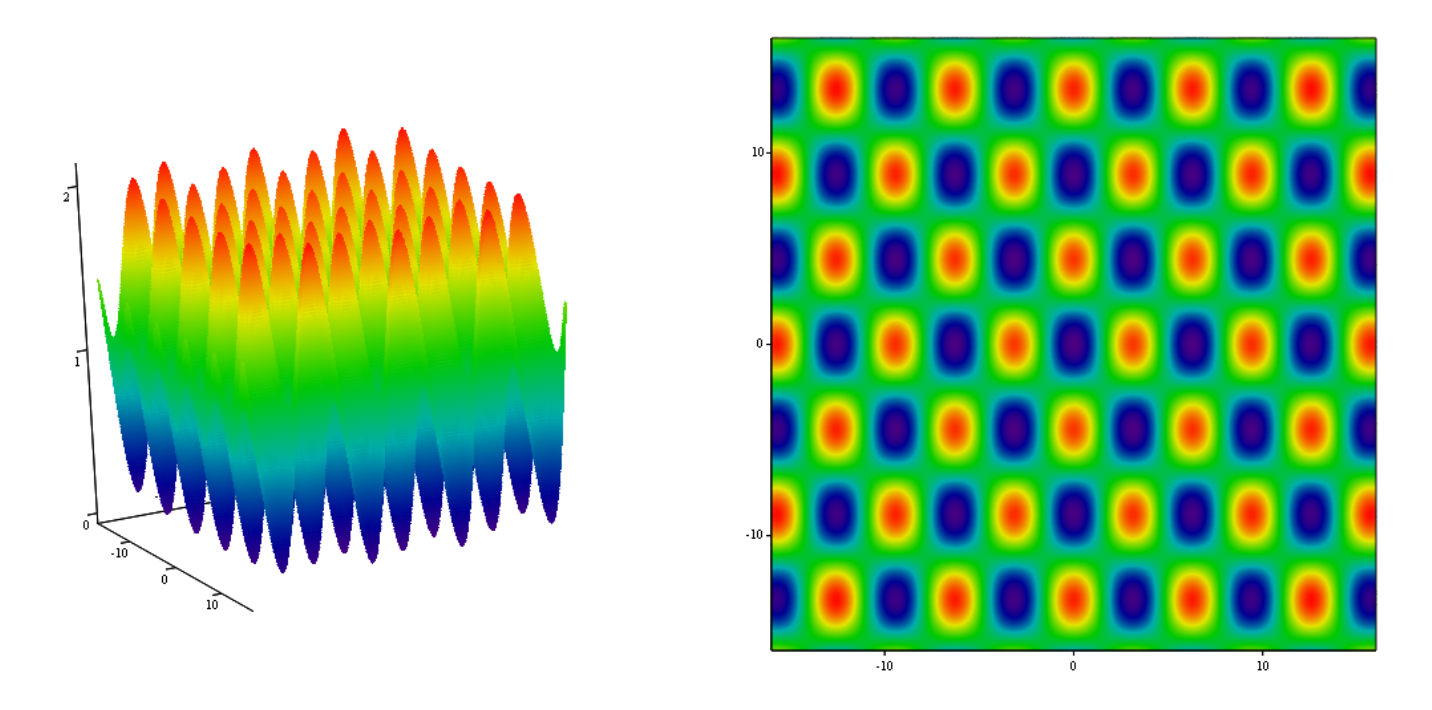
\includegraphics[width=16cm, height=8cm]{Grivank}

    \subsubsection*{Формула}
    \begin{gather*}
        f(x)=\sum_{i=1}^n \frac{x_i^2}{4000}-\prod_{i=1}^n \cos \left(\frac{x_i}{\sqrt{i}}\right)+1
    \end{gather*}

    \subsubsection*{Результаты тестирования}

    \begin{tabular}{ |p{2cm}|p{2cm}|p{3cm}|p{2cm}|p{4cm}|  }
        \hline
        n  & точность & метод         & время   & значение               \\
        \hline
        5  & $10^-3$  & Golden ratio  & 2.41 ms & 0.009864698515380743   \\\cline{2-5}
        & $10^-3$  & Moore-Skelboe & 183 ms  & 1.0644240466817223e-07 \\
        \hline
        10 & $10^-3$  & Golden ratio  & 6.05 ms & 0.009864698515380743   \\\cline{2-5}
        & $10^-3$  & Moore-Skelboe & 739 ms  & 1.3662353537391425e-07 \\
        \hline
        20 & $10^-3$  & Golden ratio  & 21.4 ms & 0.009864698515380743   \\\cline{2-5}
        & $10^-3$  & Moore-Skelboe & 2.44 s  & 1.6799845647952338e-07 \\
        \hline
        30 & $10^-3$  & Golden ratio  & 40.2 ms & 0.009864698515380743   \\\cline{2-5}
        & $10^-3$  & Moore-Skelboe & 5.16 s  & 1.867295605917363e-07  \\
        \hline
        40 & $10^-3$  & Golden ratio  & 59.3 ms & 0.009864698515380743   \\\cline{2-5}
        & $10^-3$  & Moore-Skelboe & 9.09 s  & 2.0016648982768004e-07 \\
        \hline
        50 & $10^-3$  & Golden ratio  & 84.4 ms & 0.009864698515380743   \\\cline{2-5}
        & $10^-3$  & Moore-Skelboe & 14 s    & 2.1067470723501458e-07 \\
        \hline

    \end{tabular}

    \subsection*{Функция Швефеля}

    \subsubsection*{График функции при $n=2$}
    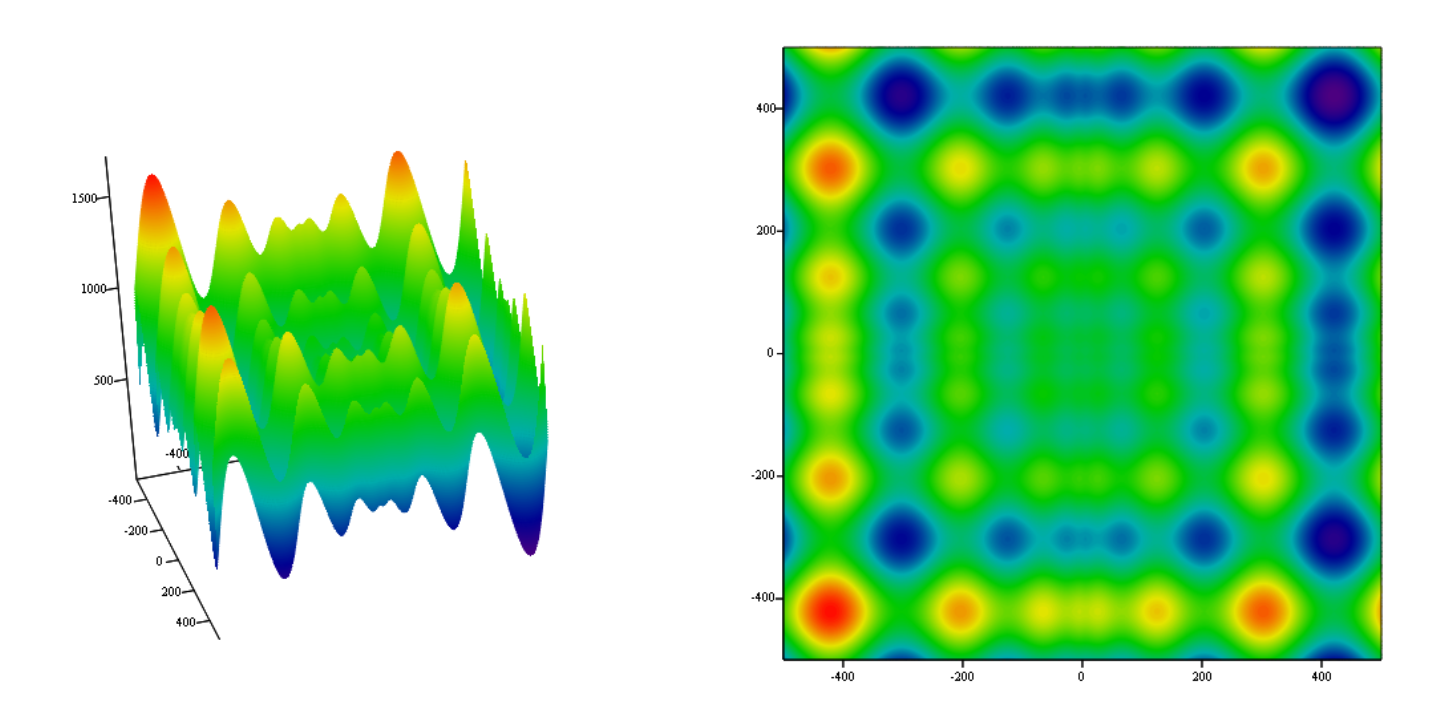
\includegraphics[width=16cm, height=8cm]{Shvefel}

    \subsubsection*{Формула}
    \begin{gather*}
        f(x)=418.9829 n-\sum_{i=1}^n\left(x_i \sin \left(\sqrt{\left|x_i\right|}\right)\right)
    \end{gather*}

    \subsubsection*{Результаты тестирования}

    \begin{tabular}{ |p{2cm}|p{2cm}|p{3cm}|p{2cm}|p{4cm}|  }
        \hline
        n & точность & метод         & время   & значение               \\
        \hline
        2 & $10^-3$  & Golden ratio  & 721 µs  & 236.8766946858181      \\\cline{2-5}
        & $10^-3$  & Moore-Skelboe & 4.98 s  & 2.5455285594944144e-05 \\
        \hline
        3 & $10^-3$  & Golden ratio  & 800 µs  & 355.3150420287272      \\\cline{2-5}
        & $10^-3$  & Moore-Skelboe & 9.41 s  & 3.8182928392416216e-05 \\
        \hline
        4 & $10^-3$  & Golden ratio  & 1.44 ms & 473.7533893716363      \\\cline{2-5}
        & $10^-3$  & Moore-Skelboe & 15 s    & 5.091057118988829e-05  \\
        \hline
        5 & $10^-3$  & Golden ratio  & 1.4 ms  & 592.1917367145454      \\\cline{2-5}
        & $10^-3$  & Moore-Skelboe & 22 s    & 6.363821398736036e-05  \\
        \hline
        6 & $10^-3$  & Golden ratio  & 2.19 ms & 710.6300840574543      \\\cline{2-5}
        & $10^-3$  & Moore-Skelboe & 31.1 s  & 7.636585655745876e-05  \\
        \hline
        7 & $10^-3$  & Golden ratio  & 1.88 ms & 829.0684314003631      \\\cline{2-5}
        & $10^-3$  & Moore-Skelboe & 40 s    & 8.909349912755715e-05  \\
        \hline
        8 & $10^-3$  & Golden ratio  & 4.92 ms & 947.5067787432718      \\\cline{2-5}
        & $10^-3$  & Moore-Skelboe & 52 s    & 0.00010182114169765555 \\
        \hline

    \end{tabular}
